%!TEX root = ../assignment1.tex

\section{Outcome}
In this section, we gather the findings of two phases of research and seek to invent a general tool for partitioner to evaluate how possible a ICT project is going to succeed.

\subsection{Analysis Of Findings}

In this section, we use mathematical approaches to investigate the correlation of the findings in both phases.

\subsubsection{Average And Standard Deviation}
In Phase 1, the average global influence score is 3.6 and standard deviation
is 2.17. In Phase 2, they are 2.66 and 1.37. It suggests the proposals in Phase 1 has more general influence on how to make ICT project successful. However, standard deviation values indicate the influence power in Phase 1 varies more than that of Phase 2.
\subsubsection{Pie Chart By Primary Themes}
To further our analysis on how primary themes(control, process, people and structure) distribute in both Phase 1 and Phase 2, we draw a pie chart to show the proportion.
% \begin{figure}[ht]
% \caption{Primary Themes in Phase 1}
% \centering
% \resizebox{\columnwidth}{!}{%
% 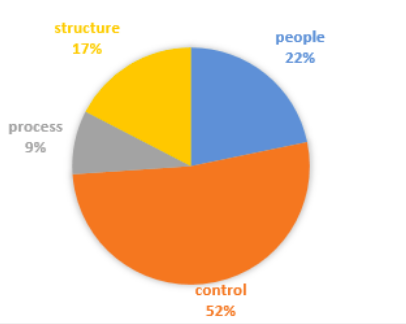
\includegraphics{pie_chart_p1.png}
% }
% \end{figure}

\begin{figure}
\centering
\begin{minipage}{.5\textwidth}
  \centering
  %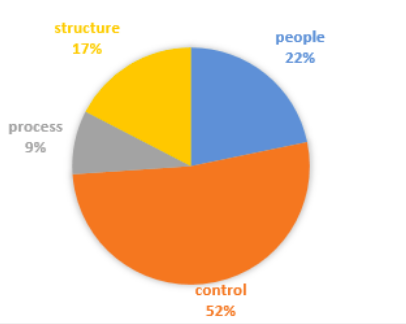
\includegraphics[width=.5\linewidth]{pie_chart_p1.png}
  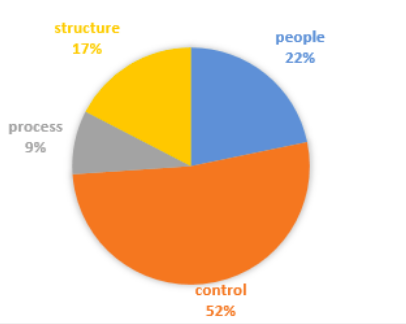
\includegraphics[height=10em]{pie_chart_p1.png}
  \captionof{figure}{Primary Themes in Phase 1}
  \label{pie:1}
\end{minipage}%
\begin{minipage}{.5\textwidth}
  \centering
  %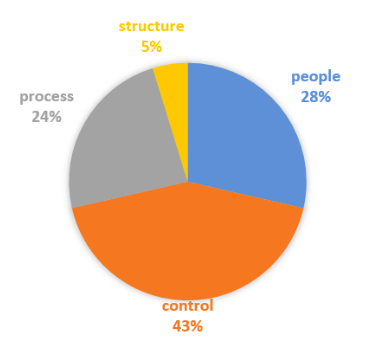
\includegraphics[width=.5\linewidth]{pie_chart_p2.png}
  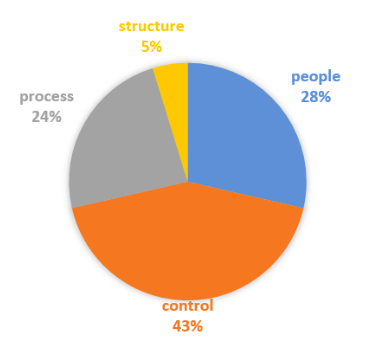
\includegraphics[height=10em]{pie_chart_p2.png}
  \captionof{figure}{Primary Themes in Phase 2}
  \label{pie:2}
\end{minipage}
\end{figure}

From the pie charts of \ref{pie:1} and \ref{pie:2}, we can conclude that the theme of control is the dominant theme of solutions followed by the theme of people, which the data of both phases agree to yield. However, there is a subtle difference in the less influential themes of process and structure. Phase 1 puts more emphasis on structure while Phase 2 puts that on process.

With the aforementioned statistical analysis, we can conclude that the findings of both Phase 1 and Phase 2 are in correlation in terms of primary themes, the values of solutions.

\subsection{Evaluation Framework}

\subsubsection{Making Of The Framework}
To convert the solutions we found into a practical tool that practitioners can use, we make our solutions into an hierarchical structure of 2 levels. The upper level is the primary themes we used in our entire research, namely control, people, process, structure. The inner level is sub-themes we find using qualitative analysis.

To find the sub-themes of the inner level, a qualitative analysis is conducted. We identify the themes by when the solution is used. There are 21 solutions for control, 11 for people, 7 for process and 5 for structure.

In control, we find the solutions can be divided into 3 categories: when planning, during implementation and when working with vendor. In people, the categories are when working with people inside same organization and when working with people outside the organization. In process, there are when designing the project and when when the project is implemented. In structure, there are when working with people inside the organization and when working with people outside the organization.

With the defined structure, we assign weights to each solution by its own global influence score in findings. We normalize the weights in percentage, which all the weights sum up to 1.

\subsubsection{The Tool}

Here is the evaluation framework we propose.

\begin{figure}[ht]
\centering
\resizebox{\columnwidth}{!}{%
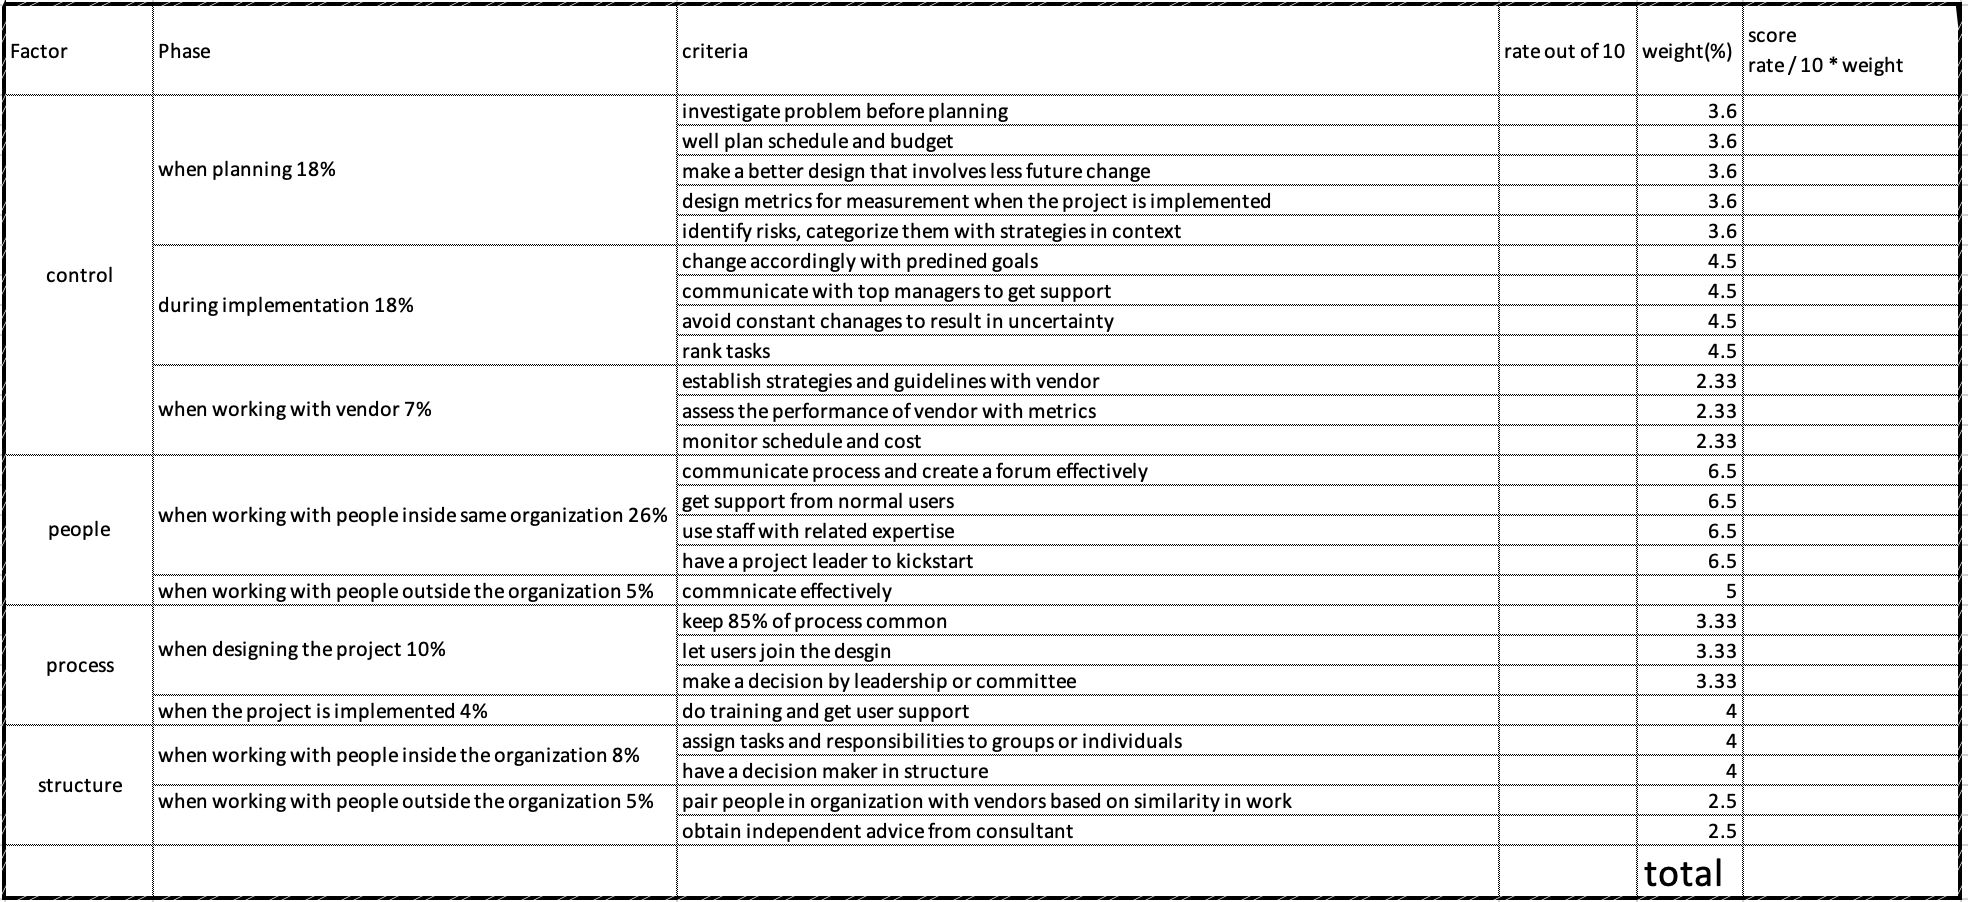
\includegraphics{tool.png}
}
\end{figure}